\section{Pose estimation}\label{sec:pose-estimation}

Pose estimation consists in detecting joint locations for persons, such ase nose, shoulders, elbows, hips... This task poses several challenges: strong articulations, small and barely visible joints, occlusions, the need to capture context.


\subsection{Human pose estimation given detection}\label{sec:pe-given-detection}

Assuming people have been already detected, and a rough bounding box is given, we can leverage information about scale and number of persons in the image. We have the advantage of disentangling detection and pose estimation, but the disadvantage of an unrealistic hypothesis.

A common practice for evaluating this task is the following:
\begin{myitem}
    \item Evaluate every key-point separately;
    \item For each person, check if key-point is correct;
    \item Compute fraction of people for which key-point is correct (\textit{Probability of Correct Key-point}).
\end{myitem}

Early methods comprise:
\begin{myitem}
    \item Graphical models with handcrafted unaries, pre-defined pairwise constraints;
    \item Pictorial structures:
    \begin{itemize}
        \item tree structured graphical models to represent spatial correlations,
        \item kinematic priors between connected limbs,
        \item occlusions, errors due to correlations outside the model;
    \end{itemize}
    \item Non-tree models:
    \begin{itemize}
        \item additional edges for symmetry, occlusion, long range interactions,
        \item can only use simpler approximate inference.
    \end{itemize}
\end{myitem}

More recent approaches use R-CNN: given an input image, extract region proposals, compute CNN features, and finally classify regions. Then there are many ways to refine proposed bounding boxes.
The first one is \textbf{Regression}:
\begin{myitem}
    \item Find and refine targets relative to bounding box;
    \item It is necessary to combine local and global appearance;
    \item \textbf{Deep networks} take whole images as input and use global information for joint regression, then regress joint locations, so there is no need to design detectors or explicitly model joint relations and spatial constraints;
    \item The objective of the network is to minimize L2 distance between the prediction and the true pose vector, and the the output is the pose vector normalized with respect to bounding box: $y^* = N^{-1} (\psi(N(x);\theta))$;
    \item On the one hand, DNs are simple and holistic, don't need to define losses to capture interactions, have hidden layers shared by joint regressors;
    \item On the other hand DNs have limited ability to consider details;
    \item With the same network architecture but different parameters (i.e. $\theta_s$) we can build a \textbf{Cascade of regressors}, where the CNN regressor at stage $s>1$ is trained with predicted joint from stage $s-1$;
    \item W.r.t. DNs, this method obtains increasingly detailed predictions along cascade stages, but can produce only one prediction per image, no candidates, and the final result depends on the quality of the initial prediction;
    \item It is also possible to consider multimodal distributions.
\end{myitem}
The second one is \textbf{Heatmaps}:
\begin{myitem}
    \item In training, each key-point is a separate binary heatmap, where the key-point is positive and the rest is negative;
    \item Possible approaches are:
    \begin{itemize}
        \item \textit{Softmax} over all locations: $p(x,y) = \frac{e^{s(x,y)}}{\sum_{x',y'} e^{s(x,y)}}$,
        \item \textit{Sigmoid} at each location: $p(x,y) = \frac{1}{1 + e^{-s(x,y)}}$;
    \end{itemize}
    \item The resolution issue may have different solutions, such as dilation, multiple layers, multiple image scales (multi-resolution feature extraction, re-utilization of convolutional features).
\end{myitem}
These methods can be combined by using heatmap to predict coarse location and then predicting an offset $(\Delta x, \Delta y)$ at each location.

It is important to consider that key-points are not all independent, given the image. For example, a person can't have right elbow and left wrist on the same arm. Thus, we have to capture \textit{key-point dependence}, with \textbf{structured prediction}: let $l$ be a candidate location for each key-point, then we have
\begin{flalign}\label{eq:keypoint-dependence}
    E(l) &= \underbrace{\sum_i s_i(l_i)}_{\substack{\text{score from} \\ \text{heatmap}}} + \underbrace{\phi(l)}_{\substack{\text{consistency} \\ \text{between joints}}}\\
    &= \sum_i s_i(l_i) + \sum_{ij} \phi_{ij} (l_i, l_j)
\end{flalign}
The optimal $l^*$ is given by
\begin{equation}
    l^* = \argmin E(l)
\end{equation}
which is a conditional random field, where $\phi$ is unknown and needs to be learned.\\
Dependence between key-points can be represented with pictorial structures, such as in figure \ref{fig:pe-pictorial-structure}.

\begin{figure}[h!]
    \centering
    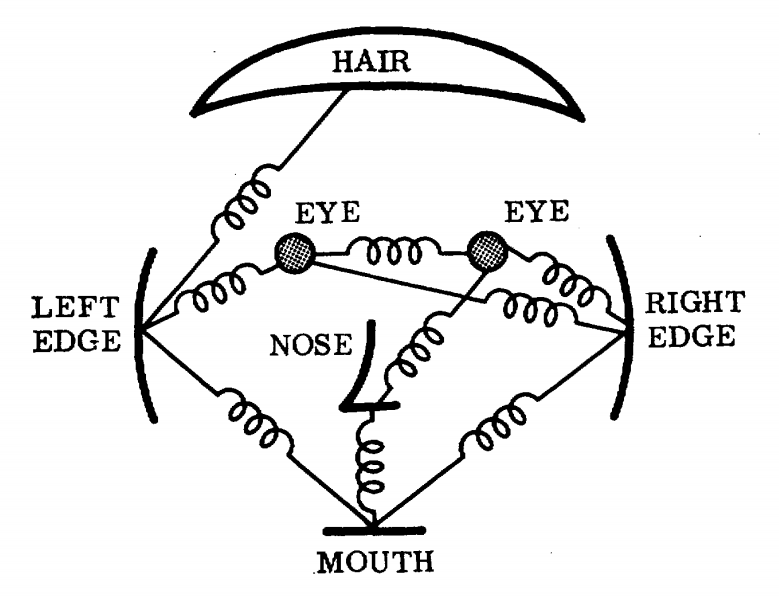
\includegraphics[width=0.4\linewidth]{images/pictorial-structure}
    \caption[Pictorial structures]{Pictorial structures}
    \label{fig:pe-pictorial-structure}
\end{figure}

Another possible approach is to learn a \textit{flexible mixture of parts}:
\begin{equation}\label{eq:mixture-parts}
    S(I,L) = \sum_{i \in V} \alpha_i \cdot \phi(I, l_i) + \sum_{ij \in E} \beta_{ij} \cdot \psi(l_i, l_j)
\end{equation}
where $\psi(l_i, l_j)$ represents spatial features between $l_i$ and $l_j$, and $\beta_{i,j}$ represents pairwise springs between part $i$ and part $j$.\\
This can be done with \textbf{structured SVMs}:
\begin{myitem}
    \item Very large output spaces,
    \item A scoring function that scores input-output pairs $h_w(x,y)$,
    \item Predicted output is $\argmax$ of the scoring function,
    \item Loss is margin rescaled loss.
\end{myitem}

So, inference is performed as follows:
\begin{flalign}
    E(l) &= \sum_i s_i(l_i) + \sum_{i,j} \phi_{i,j} (l_i, l_j)\\
    l^* &= \argmin E(l)\\
    l_i^* &= \argmin_{l_i} \left(s_i(l_i) + \sum_{j} \phi_{i,j} (l_i, l_j^*) \right)\\
    l_i^{(t+1)} &\gets \argmin_{l_i} \left(s_i(l_i) + \sum_{j} \phi_{i,j} (l_i, l_j^{(t)}) \right) \label{eq:pose-iterative}
\end{flalign}
That is, instead of learning scoring function, we apply \textbf{iterative models} to approximately minimize it. This approach is similar to Inference machines and Autocontext (the former share the parameters, the latter don't - see figures \ref{fig:pe-inference-machine} and \ref{fig:pe-autocontext}).

\begin{minipage}{.66\linewidth}
\begin{figure}[H]
    \centering
    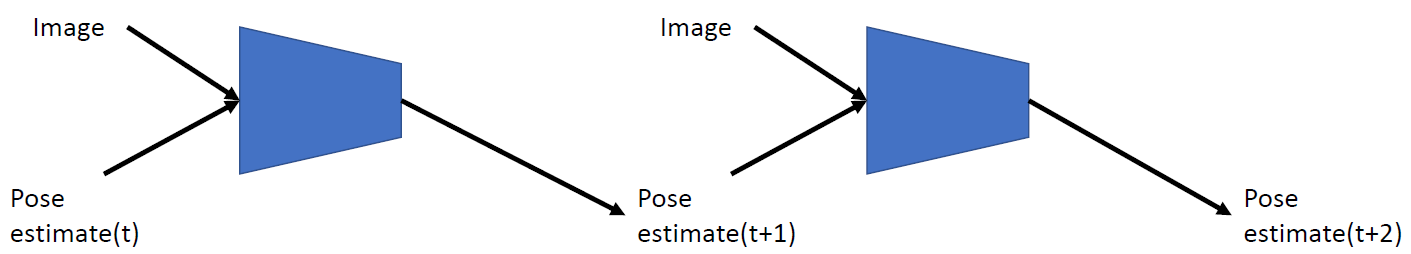
\includegraphics[width=0.7\linewidth]{images/inference-machine}
    \caption[Inference machine]{Inference machine}
    \label{fig:pe-inference-machine}
\end{figure}
\end{minipage}
\begin{minipage}{.33\linewidth}
\begin{figure}[H]
    \centering
    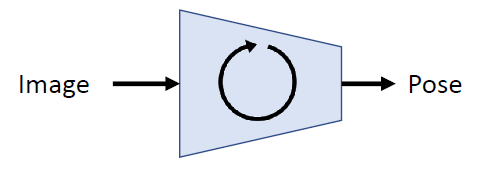
\includegraphics[width=0.7\linewidth]{images/autocontext}
    \caption[Autocontext]{Autocontext}
    \label{fig:pe-autocontext}
\end{figure}
\end{minipage}

Going into more detail:
\begin{myitem}
    \item In each iteration, beliefs of one variable are updated using current beliefs of the others, according to equation \ref{eq:pose-iterative};
    \item Frame each iteration of inference as a differentiable function;
    \item Write inference as a convolutional network.
\end{myitem}

For example:
\begin{myitem}
    \item $P(\text{eye at } p) = \sum_q P(\text{eye at } p | \text{nose at } q)$,
    \item $P(\text{eye at } p | \text{nose at } q)$ only depends on relative location of $p$ and $q$,
    \item $f(p) = \sum_q w(p-q)g(q)$: convolution,
    \item $f = w \cdot g$.
\end{myitem}

\begin{figure}[h!]
    \centering
    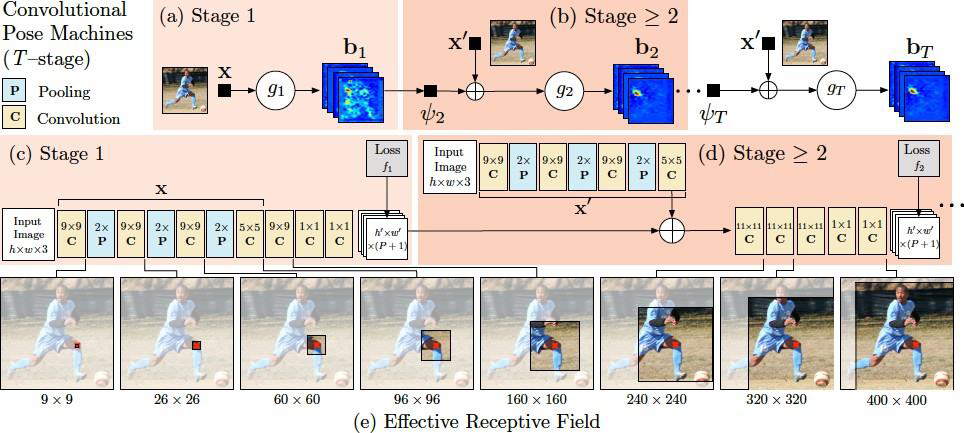
\includegraphics[width=0.7\linewidth]{images/convolutional-pose-machine}
    \caption[Convolutional Pose Machine]{Convolutional Pose Machine}
    \label{fig:pe-convolutional-pose-machine}
\end{figure}

Differently from other models such as \textbf{FLIC} or \textbf{LSP}, in \textbf{Convolutional Pose Machines} each iteration can involve multiple convolution/subsampling layers over beliefs from previous iteration. In this network (see figure \ref{fig:pe-convolutional-pose-machine}), each stage sees two inputs: image features and context features (based on output from previous stage). Its goal is to achieve large receptive fields to learn complex and long range interactions.\\
First stage:
\begin{myitem}
    \item Predict part belief based on local image values;
    \item Output $P+1$ heat maps ($P$ for parts and 1 for background);
    \item Small receptive field, to capture relation between close parts (e.g. between head and shoulders, but not head and knees).
\end{myitem}
Following stages:
\begin{myitem}
    \item Image features $x'$ from the previous stage;
    \item Context function $\psi$ encodes landscape of belief maps around part locations ($\psi$ is the receptive field, actually);
    \item In this way, the network decides how to combine features and learn higher relations, and hand-defined graphical models are no more needed;
    \item Receptive field size can be increased by more pooling (with loss of local details), larger filters (but the number of parameters increases) or more layers (with vanishing gradient problem).
\end{myitem}
Since magnitude of backpropagated gradients decreases rapidly in initial layers, intermediate supervision are used to ensure greater variance in gradients.

\begin{minipage}{.5\linewidth}
    \begin{figure}[H]
        \centering
        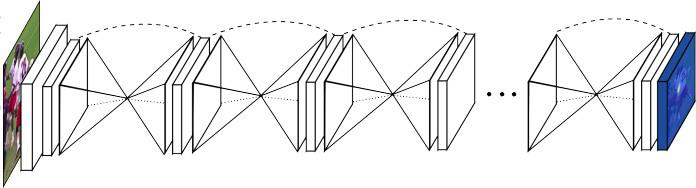
\includegraphics[width=0.95\linewidth]{images/staked-hourglass}
        \caption[Staked Hourglass Network (a)]{Staked Hourglass Network (a)}
        \label{fig:pe-stacked-hourglass}
    \end{figure}
\end{minipage}
\begin{minipage}{.5\linewidth}
    \begin{figure}[H]
        \centering
        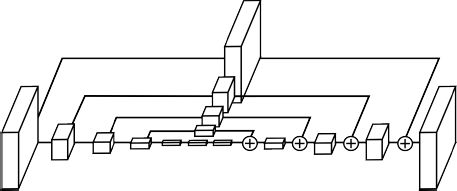
\includegraphics[width=0.95\linewidth]{images/staked-hourglass1}
        \caption[Staked Hourglass Network (b)]{Staked Hourglass Network (b)}
        \label{fig:pe-stacked-hourglass1}
    \end{figure}
\end{minipage}

An alternative model, which can be used for this task, is the \textbf{Stacked Hourglass Network}. As the name suggests, and as figure \ref{fig:pe-stacked-hourglass} shows, it has a ``hourglass structure''. Each refinement round has to combine global information about pose, and use this information to produce new precise pose estimate. Moreover, rounds don't need to share parameters.\\
This network combine local appearance, needed for accurate part detection, with global reasoning, useful for orientation of body, limb arrangement and part relationships. It is designed to process multiple scales and achieve pixel-wise predictions, by applying convolution and max-pooling to very low $4 \times 4$ resolution and then upsampling and combining with skip connection (see figure \ref{fig:pe-stacked-hourglass1}). The refinement is obtained through iterative stages, by reducing and augmenting resolution. It is also possible to apply intermediate supervision for each stage:
\begin{myitem}
    \item Network has had a chance to reason both locally and globally,
    \item Subsequent hourglass modules can reassess high order spatial relations,
    \item Ask network to repeatedly reason across scales,
    \item 1x1 convolution to add intermediate heatmaps to feature channels.
\end{myitem}
Stacked (cascading) hourglass is better than long hourglass, which, in turn, is better than short hourglass. Furthermore, intermediate supervision helps both single an stacked models.


\subsection{Human pose estimation without detection}\label{sec:pe-without-detection}

Without any assumption about detection, we have no idea of the scale or the number of persons in the image. This can be also an opportunity: we can leverage key-point estimates to improve detections. We have the advantage of a more realistic scenario, but the disadvantage of conflating detection and pose estimation.

There are two different approaches to human pose estimation without detection: top-down and bottom-up.


\subsubsection{Top-Down pose estimation}\label{sec:pe-top-down}

The key idea of this approach is \textit{detect people, then estimate their parts}.\\
In this case, it is possible to use any of the technique described in section \ref{sec:pe-given-detection}, the problem is similar to instance segmentation, it is easy to get object level information, but hard to recover from bad detections.

An example of network to perform this task is \textbf{Mask R-CNN}, shown in figure \ref{fig:pe-mask-r-cnn} (see section \ref{sec:ds-instance}).

\begin{figure}[h!]
    \centering
    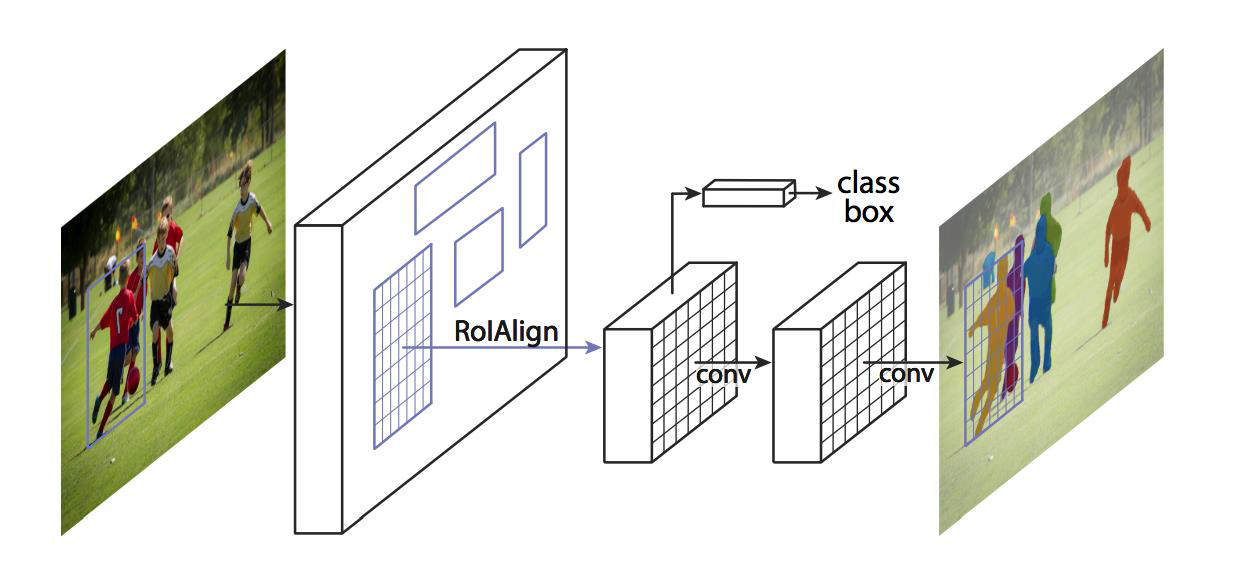
\includegraphics[width=0.7\linewidth]{images/mask-r-cnn}
    \caption[Mask R-CNN]{Mask R-CNN}
    \label{fig:pe-mask-r-cnn}
\end{figure}


\subsubsection{Bottom-Up pose estimation}\label{sec:pe-bottom-up}

The key idea of this approach is \textit{detect parts, then associate those to people}.\\
In this case, we need a way to group joints, which is a hard problem, due to its inherent ambiguity, and requires heuristics; moreover, there is no simple way to have object level information.

\textbf{Realtime Multi Person 2D Pose Estimation using Part Affinity Fields} is a technique that uses detection of limbs and limb orientation to guide the key-point grouping. The novelty introduced by this method is to jointly learn parts detection and parts association, through a single CNN.\\
Parts detection is based on \textit{sequential prediction with learned spatial context}: stage by stage, each key-point is found, and finding the previous one helps finding the next one. For this reason, it is useful to find the easier parts first, then the harder ones.\\
Part-to-part and Part-to-person association is guided by the \textit{affinity score}. Since the part affinity score is dependent on visual appearance, it can be encoded on the image plane: \textit{part affinity fields} encode direction and position of body parts, which are used to determine the affinity score, which in turn helps to define the midpoint score map for part-to-part association and the part-to-part association itself, and to reduce spatial ambiguities. Part affinity fields are learned in parallel with parts detection by the second branch of the network, as shown in figure \ref{fig:pe-affinity-fields}.

\begin{figure}[h!]
    \centering
    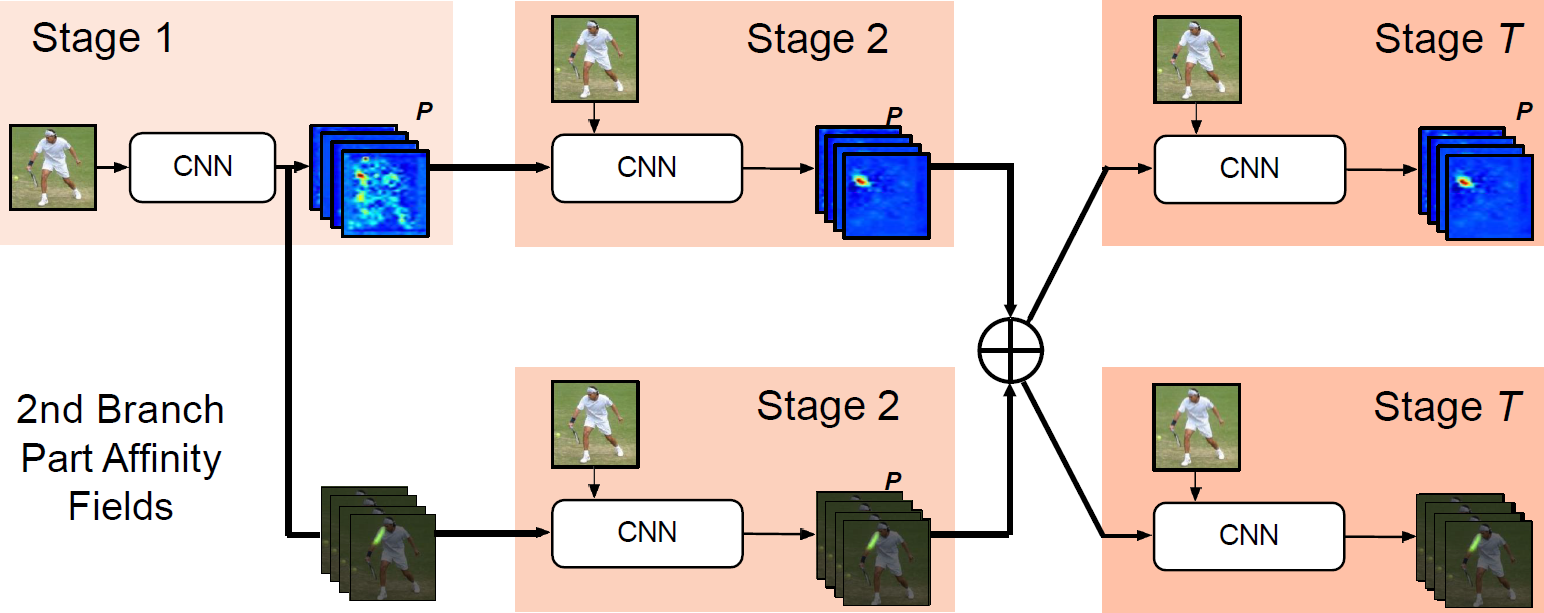
\includegraphics[width=0.7\linewidth]{images/affinity-fields}
    \caption[Pose Estimation using Part Affinity Fields (architecture)]{Pose Estimation using Part Affinity Fields (architecture}
    \label{fig:pe-affinity-fields}
\end{figure}
\begin{figure}[h!]
    \centering
    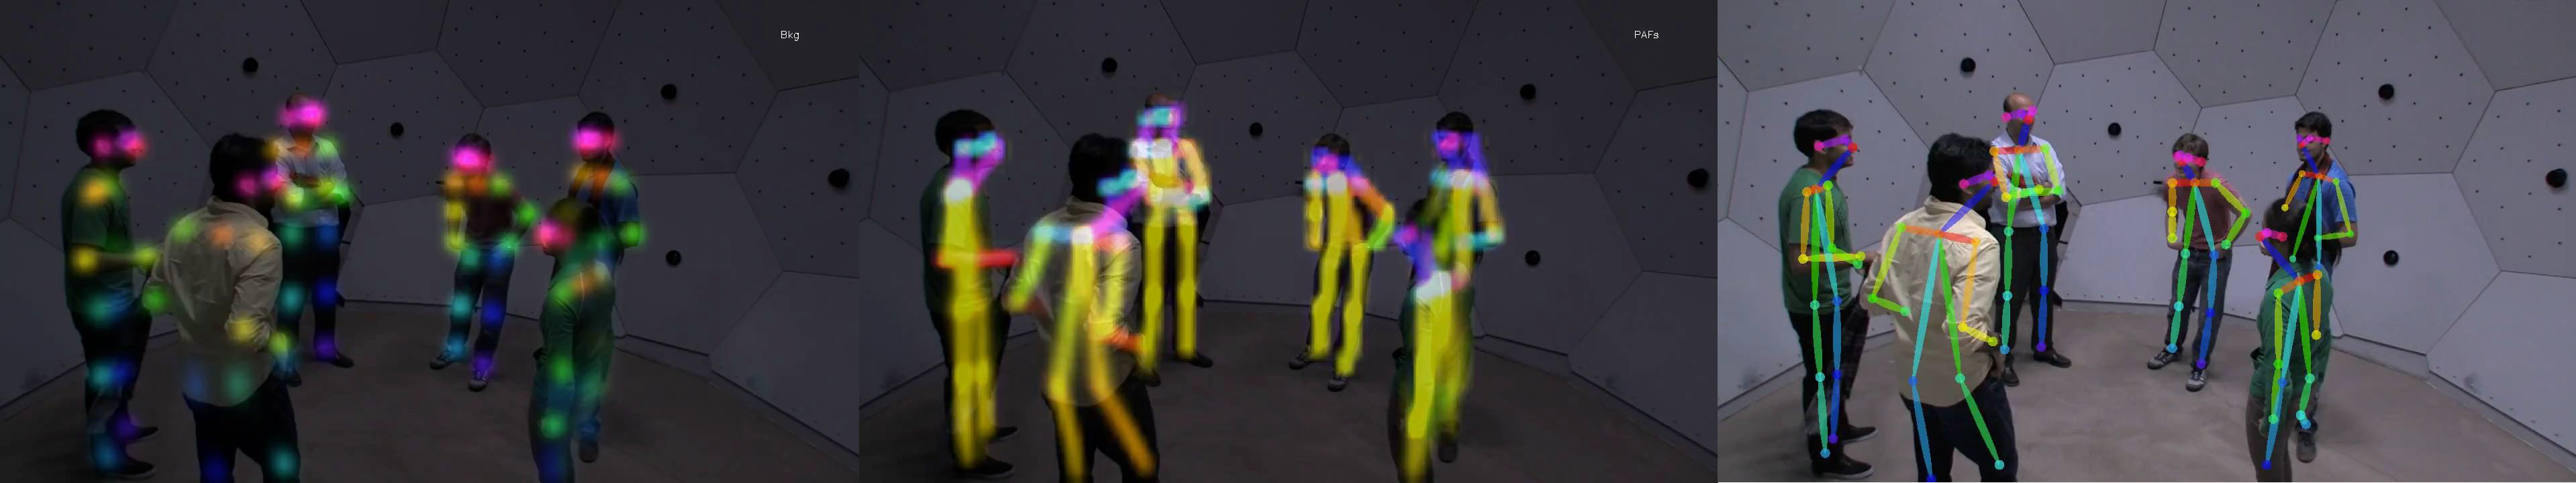
\includegraphics[width=\linewidth]{images/affinity-fields-1}
    \caption[Pose Estimation using Part Affinity Fields (application example)]{Pose Estimation using Part Affinity Fields (application example)}
    \label{fig:pe-affinity-fields-1}
\end{figure}


\newpage
\subsection{3D pose estimation of people and objects}\label{sec:pe-3d}

To do pose estimation in 3D, we need to know relative lengths of each limb. The basic assumption is \textit{scaled orthographic projection}, that is, we don't need to know the exact depth of each limb, we can approximate it \textit{if} variation in depth is very smaller than depth, i.e., if the whole person is almost at the same distance from the camera. In math terms:
\begin{flalign}\label{eq:3d-pose}
    x &= \frac{X}{Z} \approx \frac{X}{Z_0}\\
    y &= \frac{Y}{Z} \approx \frac{Y}{Z_0}
\end{flalign}
with $Z_0$ constant.\\
The relative depth between two points $(X_1, Y_1, Z_1)$ and $(X_2, Y_2, Z_2)$, called $d_Z$, is computed as follows:
\begin{flalign}\label{eq:relative-depth}
    l^2 &= (X_1-X_2)^2 + (Y_1-Y_2)^2 + (Z_1-Z_2)^2\\
    (u_1-u_2) &= s(X_1 - X_2)\\
    (v_1-v_2) &= s(Y_1 - Y_2)\\
    d_Z = (Z_1 - Z_2) &= \sqrt{l^2 - \frac{(u_1-u_2)^2 + (v_1-v_2)^2}{s^2}}
\end{flalign}

Pose estimation for rigid objects is easier than for people, since they have fixed shape. The goal, in this case, is to understand position and orientation of the key-points of the objects (e.g. the wheels of a car). In other words, we're interested in capturing the ``six degrees of freedom'' of the object, that is, its $X,Y,Z$ position, plus its roll (cyclo-rotation), its pitch (elevation) and its yaw (azimuth). To do that, we try to minimize the \textit{reprojection error}, i.e., the distance between the ground truth and the key-points detected and reprojected on the plane. The best way to fit viewpoint to key-points would be to have canonical frames for each object (e.g. CAD models) which provide 3D location of each key-point, but too many models would be needed. Thus, we just use simplified models for classes of objects, or represent objects as combination of basic shapes (analogously to what we do with Fourier transforms for waves).
